% ------------------------------------------------------------------------------
% TYPO3 Version 10.1 - What's New (Italian Version)
%
% @license	Creative Commons BY-NC-SA 3.0
% @link		http://typo3.org/download/release-notes/whats-new/
% @language	Italian
% ------------------------------------------------------------------------------

\section{Modifiche per sviluppatori}
\begin{frame}[fragile]
	\frametitle{Modifiche per sviluppatori}

	\begin{center}\huge{Capitolo 3:}\end{center}
	\begin{center}\huge{\color{typo3darkgrey}\textbf{Modifiche per sviluppatori}}\end{center}

\end{frame}

% ------------------------------------------------------------------------------
% Feature | 89054 | Provide core cache frontends via dependency injection

\begin{frame}[fragile]
	\frametitle{Modifiche per sviluppatori}
	\framesubtitle{Injection delle dipendenze della Cache (1)}

	% decrease font size for code listing
	\lstset{basicstyle=\tiny\ttfamily}

	\begin{itemize}
		\item Gli sviluppatori di Estensioni sono incoraggiati a fare direttamente injection della Cache, anziché utilizzare CacheManager.
		\item Questo richiede alcune piccole modifiche come mostrato di seguito.

		\item \textbf{In precedenza:}

\begin{lstlisting}
class MyClass
{
  /**
   * @var TYPO3\CMS\Core\Cache\Frontend\FrontendInterface
   */
  private $cache;

  public function __construct()
  {
      $cacheManager = GeneralUtility::makeInstance(CacheManager::class);
      $this->cache = $cacheManager->getCache('my_cache');
  }
}
\end{lstlisting}

	\end{itemize}

\end{frame}

% ------------------------------------------------------------------------------
% Feature | 89054 | Provide core cache frontends via dependency injection

\begin{frame}[fragile]
	\frametitle{Modifiche per sviluppatori}
	\framesubtitle{Injection delle dipendenze della Cache (2)}

	% decrease font size for code listing
	\lstset{basicstyle=\tiny\ttfamily}

	\begin{itemize}
		\item Da \textbf{TYPO3 v10.1}, la classe deve apparire come segue:

\begin{lstlisting}
class MyClass
{
  /**
   * @var TYPO3\CMS\Core\Cache\Frontend\FrontendInterface
   */
  private $cache;

  public function __construct(FrontendInterface $cache)
  {
    $this->cache = $cache;
  }
}
\end{lstlisting}

	\end{itemize}

\end{frame}

% ------------------------------------------------------------------------------
% Feature | 89054 | Provide core cache frontends via dependency injection

\begin{frame}[fragile]
	\frametitle{Modifiche per sviluppatori}
	\framesubtitle{Injection delle dipendenze della Cache (3)}

	% decrease font size for code listing
	\lstset{basicstyle=\tiny\ttfamily}

	\begin{itemize}
		\item ...ed è richiesta la seguente configurazione del servizio container:

\begin{lstlisting}
services:
  cache.my_cache:
    class: TYPO3\CMS\Core\Cache\Frontend\FrontendInterface
    factory: ['@TYPO3\CMS\Core\Cache\CacheManager', 'getCache']
    arguments: ['my_cache']

  MyClass:
    arguments:
      $cache: '@cache.my_cache'
\end{lstlisting}

	\end{itemize}

\end{frame}

% ------------------------------------------------------------------------------
% Feature | 89066 | Add PHP API for Notifications in backend
%
%\begin{frame}[fragile]
%	\frametitle{Changes for Developers}
%	\framesubtitle{Backend Notifications}
%
%	% decrease font size for code listing
%	\lstset{basicstyle=\smaller\ttfamily}
%
%	\begin{itemize}
%		\item A new PHP API provides a simple way to create JavaScript backend notifications.
%		\item For example:
%
%\begin{lstlisting}
%GeneralUtility::makeInstance(NotificationService::class)
%   ->notice('Notice', 'notice');
%\end{lstlisting}
%
%	\end{itemize}
%
%	\begin{figure}
%		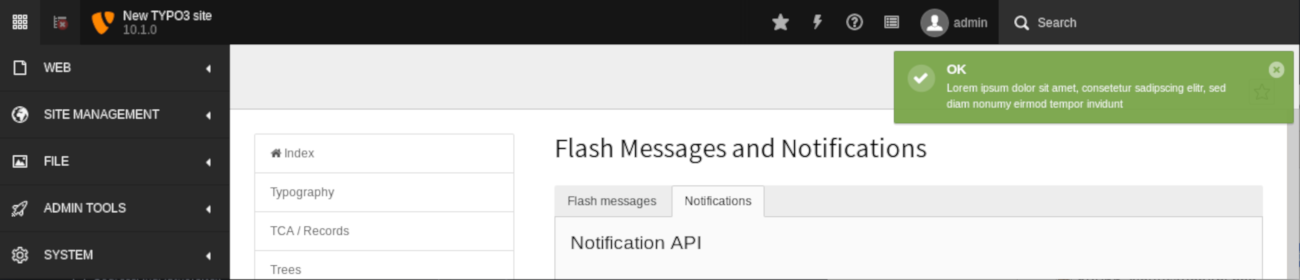
\includegraphics[width=0.90\linewidth]{ChangesForDevelopers/89066-NotificationApi.png}
%	\end{figure}
%
%\end{frame}

% ------------------------------------------------------------------------------
% Feature | 89061 | Introduce Notification Actions

\begin{frame}[fragile]
	\frametitle{Modifiche per sviluppatori}
	\framesubtitle{Azioni di notifica}

	\begin{itemize}
		\item Le notifiche JavaScript nel backend dispongono di azioni (bottoni).
	\end{itemize}

	\begin{figure}
		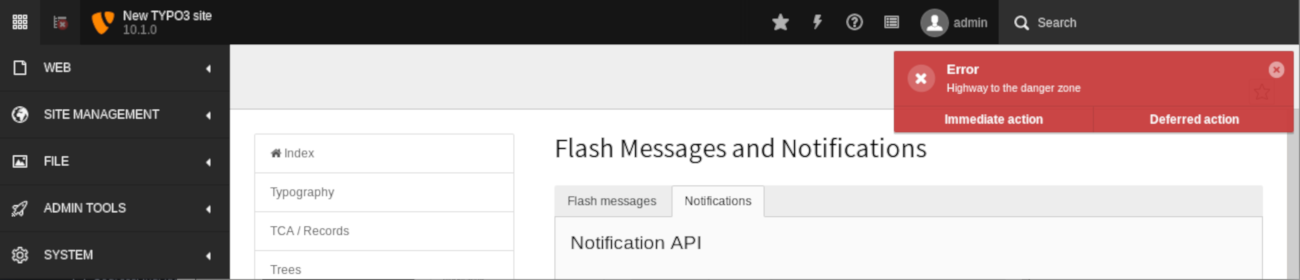
\includegraphics[width=0.90\linewidth]{ChangesForDevelopers/89061-NotificationActionsAndButtons.png}
	\end{figure}

\end{frame}

% ------------------------------------------------------------------------------
% Feature | 89244 | Broadcast Channels and Messaging

\begin{frame}[fragile]
	\frametitle{Modifiche per sviluppatori}
	\framesubtitle{Canali di trasmissione e messaggistica (1)}

	% decrease font size for code listing
	\lstset{basicstyle=\tiny\ttfamily}

	\begin{itemize}
		\item E' possibile inviare e ricevere "messaggi" usando JavaScript.
	\end{itemize}

	\vspace{-0.2cm}
	\begingroup
		\color{red}
			\begin{center}
				L'API è attualmente considerata \textbf{internal} è può cambiare\newline
				in qualsiasi momento fino a quando non viene dichiarata "stabile".
			\end{center}
	\endgroup

	\begin{itemize}
		\item Esempio per \textbf{inviare} un messaggio:

\begin{lstlisting}
require(['TYPO3/CMS/Backend/BroadcastService'], function (BroadcastService) {
  const payload = {
    componentName: 'my_extension',
    eventName: 'my_event',
    foo: 'bar'
  };
  BroadcastService.post(payload);
});
\end{lstlisting}

	\end{itemize}

\end{frame}

% ------------------------------------------------------------------------------
% Feature | 89244 | Broadcast Channels and Messaging

\begin{frame}[fragile]
	\frametitle{Modifiche per sviluppatori}
	\framesubtitle{Canali di trasmissione e messaggistica (2)}

	% decrease font size for code listing
	\lstset{basicstyle=\tiny\ttfamily}

	\begin{itemize}
		\item Esempio per \textbf{ricevere} un messaggio:

\begin{lstlisting}
define([], function() {
  document.addEventListener('typo3:my_component:my_event', (e) => eventHandler(e.detail));
  function eventHandler(detail) {
    // output contains key 'foo' as the payload
    console.log(detail);
  }
});
\end{lstlisting}

		\item Vedi \href{https://developer.mozilla.org/en-US/docs/Web/API/Broadcast_Channel_API}{developer.mozilla.org} per maggiori informazioni.

	\end{itemize}

\end{frame}

% ------------------------------------------------------------------------------
% Feature | 89018 | Provide implementation for PSR-17 HTTP Message Factories

\begin{frame}[fragile]
	\frametitle{Modifiche per sviluppatori}
	\framesubtitle{PSR-17 HTTP Message Factories}

	\begin{itemize}
		\item E' stato implementato \href{https://www.php-fig.org/psr/psr-17/}{PSR-17}
			HTTP Message Factories.
		\item Le interfacce HTTP Message Factory devono essere utilizzate come dipendenze
			per gestori di richieste o servizi che creano oggetti di tipo messaggio PSR-7.
		\item PSR-17 è costituito da sei interfacce:

			\begin{itemize}\smaller
				\item \texttt{\textbackslash
					Psr\textbackslash
					Http\textbackslash
					Message\textbackslash
					RequestFactoryInterface}
				\item \texttt{\textbackslash
					Psr\textbackslash
					Http\textbackslash
					Message\textbackslash
					ResponseFactoryInterface}
				\item \texttt{\textbackslash
					Psr\textbackslash
					Http\textbackslash
					Message\textbackslash
					ServerRequestFactoryInterface}
				\item \texttt{\textbackslash
					Psr\textbackslash
					Http\textbackslash
					Message\textbackslash
					StreamFactoryInterface}
				\item \texttt{\textbackslash
					Psr\textbackslash
					Http\textbackslash
					Message\textbackslash
					UploadedFileFactoryInterface}
				\item \texttt{\textbackslash
					Psr\textbackslash
					Http\textbackslash
					Message\textbackslash
					UriFactoryInterface}

			\end{itemize}\normalsize

		\item Vedi la
			\href{https://docs.typo3.org/c/typo3/cms-core/master/en-us/Changelog/10.1/Feature-89018-ProvideImplementationForPSR-17HTTPMessageFactories.html}{documentazione}
			per codice di esempio.

	\end{itemize}

\end{frame}

% ------------------------------------------------------------------------------
% Feature | 89216 | PSR-18 HTTP Client Implementation

\begin{frame}[fragile]
	\frametitle{Modifiche per sviluppatori}
	\framesubtitle{PSR-18 HTTP Client}

	\begin{itemize}
		\item E' stata aggiunta l'implementazione del client HTTP \href{https://www.php-fig.org/psr/psr-18/}{PSR-18}.
		\item Permette agli sviluppatori di generare richieste HTTP basate su oggetti messaggio PSR-7
			senza fare riferimento ad un'implementazione client HTTP specifica.
		\item Non sostituisce l'attuale wrapper \href{http://guzzlephp.org/}{Guzzle},
		    ma fornisce un'alternativa più generica.
		\item PSR-18 è costituito da interfacce client e tre interfacce di Exception:

			\begin{itemize}\smaller
				\item \texttt{\textbackslash
					Psr\textbackslash
					Http\textbackslash
					Client\textbackslash
					ClientInterface}
				\item \texttt{\textbackslash
					Psr\textbackslash
					Http\textbackslash
					Client\textbackslash
					ClientExceptionInterface}
				\item \texttt{\textbackslash
					Psr\textbackslash
					Http\textbackslash
					Client\textbackslash
					NetworkExceptionInterface}
				\item \texttt{\textbackslash
					Psr\textbackslash
					Http\textbackslash
					Client\textbackslash
					RequestExceptionInterface}
			\end{itemize}\normalsize

		\item Vedi la
			\href{https://docs.typo3.org/c/typo3/cms-core/master/en-us/Changelog/10.1/Feature-89216-PSR-18HTTPClientImplementation.html}{documentazione}
			per codice di esempio.

	\end{itemize}

\end{frame}

% ------------------------------------------------------------------------------
% Feature | 88871 | Handle middleware handler in RequestFactory correctly

\begin{frame}[fragile]
	\frametitle{Modifiche per sviluppatori}
	\framesubtitle{Gestore Middleware RequestFactory}

	% decrease font size for code listing
	\lstset{basicstyle=\tiny\ttfamily}

	\begin{itemize}
		\item E' possibile definire gestori di middleware personalizzati come un array.
		\item RequestFactory crea uno stack di gestori basato su array\newline
			\small
				\texttt{\$GLOBALS['TYPO3\_CONF\_VARS']['HTTP']['handler']}
			\normalsize
			e fa l'inject nel client.
		\item Ad esempio:

\begin{lstlisting}
use \TYPO3\CMS\Core\Utility\GeneralUtility;
use \Vendor\MyExtension\Middleware\Guzzle\CustomMiddleware;
use \Vendor\MyExtension\Middleware\Guzzle\SecondCustomMiddleware;

# Add custom middleware to default Guzzle handler stack
$GLOBALS['TYPO3_CONF_VARS']['HTTP']['handler'][] =
  (GeneralUtility::makeInstance(CustomMiddleware::class))->handler();
$GLOBALS['TYPO3_CONF_VARS']['HTTP']['handler'][] =
  (GeneralUtility::makeInstance(SecondCustomMiddleware::class))->handler();
\end{lstlisting}

	\end{itemize}

\end{frame}

% ------------------------------------------------------------------------------
% Feature | 88602 | Allow registering additional file processors

\begin{frame}[fragile]
	\frametitle{Modifiche per sviluppatori}
	\framesubtitle{Processori di file personalizzati}

	% decrease font size for code listing
	\lstset{basicstyle=\tiny\ttfamily}

	\begin{itemize}
		\item Gli sviluppatori possono registrare i propri processori di file.
		\item Aggiungi il seguente codice al file \texttt{ext\_localconf.php}:

\begin{lstlisting}
$GLOBALS['TYPO3_CONF_VARS']['SYS']['fal']['processors']['ExampleImageProcessor'] = [
  'className' => \Vendor\MyExtension\Resource\Processing\ExampleImageProcessor::class,
  'before' => 'LocalImageProcessor',
];
\end{lstlisting}

		\item Casi d'uso tipici:

			\begin{itemize}
				\item aggiungere un watermark alle immagini
				\item comprimere i file caricati in un archivio ZIP
				\item salvare copie modificate di immagini
				\item ecc.
			\end{itemize}

	\end{itemize}

\end{frame}

% ------------------------------------------------------------------------------
% Feature | 88995 | Calling registerPlugin with vendor name

\begin{frame}[fragile]
	\frametitle{Modifiche per sviluppatori}
	\framesubtitle{Extbase e Fluid}

	% decrease font size for code listing
	\lstset{basicstyle=\smaller\ttfamily}

	\begin{itemize}
		\item Ometti il nome del fornitore quando registri plugin con\newline
			\smaller
				\texttt{\textbackslash
					TYPO3\textbackslash
					CMS\textbackslash
					Extbase\textbackslash
					Utility\textbackslash
					ExtensionUtility::registerPlugin()}
			\normalsize

		\item Per esempio, usa "\texttt{Form}" invece di "\texttt{TYPO3.CMS.Form}"\newline
			\small(primo argomento)\normalsize

\begin{lstlisting}
\TYPO3\CMS\Extbase\Utility\ExtensionUtility::registerPlugin(
  'Form',
  'Formframework',
  'Form',
  'content-form',
);
\end{lstlisting}

	\end{itemize}

\end{frame}

% ------------------------------------------------------------------------------
% Important | 89001 | TSFE->createHashBase
% Feature | 89150 | Add events before and after rollback of record history entries

\begin{frame}[fragile]
	\frametitle{Modifiche per sviluppatori}
	\framesubtitle{Varie (1)}

	\begin{itemize}
		\item L'\texttt{hashParameters} per il calcolo di hashBase sono state modificati nella seguente classe:\newline
			\small
				\texttt{TYPO3\textbackslash
					CMS\textbackslash
					Frontend\textbackslash
					Controller\textbackslash
					TypoScriptFrontendController}
			\normalsize

			\begin{itemize}
				\item \texttt{gr\_list} è stato sostituito da \texttt{groupIds}.
				\item \texttt{cHash} è stato sostituito da \texttt{dynamicArguments}.
				\item \texttt{domainStartPage} è stato sostituito da \texttt{site} (identificatore sito).
			\end{itemize}

		\item Vengono inviati due nuovi eventi quando si esegue il rollback dei record:

			\begin{itemize}\smaller
				\item \texttt{TYPO3\textbackslash
					CMS\textbackslash
					Backend\textbackslash
					History\textbackslash
					Event\textbackslash
					BeforeHistoryRollbackStartEvent}
				\item \texttt{TYPO3\textbackslash
					CMS\textbackslash
					Backend\textbackslash
					History\textbackslash
					Event\textbackslash
					AfterHistoryRollbackFinishedEvent}
			\end{itemize}\normalsize

	\end{itemize}

\end{frame}

% ------------------------------------------------------------------------------
% Feature | 88805 | Add type to TYPO3/CMS/Core/Database/Query/QueryBuilder::set()

\begin{frame}[fragile]
	\frametitle{Modifiche per sviluppatori}
	\framesubtitle{Varie (2)}

	\begin{itemize}
		\item Il metodo \texttt{set()} di Query Builder ora accetta un quarto argomento
			per specificare il tipo del parametro indicato:\newline
			\small
				\texttt{TYPO3\textbackslash
					CMS\textbackslash
					Core\textbackslash
					Database\textbackslash
					Query\textbackslash
					QueryBuilder::set()}
			\normalsize\newline
			\vspace{0.2cm}
			(il default è \texttt{\textbackslash PDO::PARAM\_STR})

	\end{itemize}

\end{frame}

% ------------------------------------------------------------------------------
